\documentclass[10pt,oneside,twocolumn,a4paper]{article}

\usepackage{graphicx}
\usepackage[footnotesize,bf]{caption}
\usepackage{fancyhdr}
\usepackage[numbers,sort&compress]{natbib}
\usepackage[usenames,dvipsnames]{color}
\usepackage{sidecap_pat}
\usepackage[colorlinks=true, linkcolor=BrickRed, citecolor=Blue, urlcolor=Blue, filecolor=Blue]{hyperref}
\input{jdefs.tex}

\addtolength{\topmargin}{-.05in}
\addtolength{\textheight}{0.1in}

\fancyhead[LE,RO]{\thepage}
\fancyhead[LO,RE]{\slshape Pat Scott}
\fancyhead[C]{Banting PDF Research Proposal}
\fancyfoot[C]{}
\renewcommand{\headrulewidth}{0.4pt}
\renewcommand{\footrulewidth}{0pt}
\pagestyle{fancy}

\bibliographystyle{JHEP_pat}
\bibpunct{[}{]}{,}{n}{ }{,}

\author{Pat Scott}
\date{}

\begin{document}

\twocolumn[
\centerline{\huge Discovery and discrimination of models for new physics}
\smallskip
\centerline{\huge with combined terrestrial and astrophysical data}
\bigskip
\centerline{\Large Pat Scott}
\bigskip\bigskip]

\thispagestyle{fancy}




\subsubsection*{Core Research Questions}

\begin{itemize}
\item What is the correct theory of matter beyond the Standard Model of particle physics?  
\item What is dark matter?
\item What does simultaneous consideration of terrestrial and astrophysical data tell us about physics at the TeV energy scale?
\end{itemize}

\subsubsection*{Overview}

The identity of dark matter and the nature of physics at the TeV energy scale are two of the most pressing and fundamental questions in modern physics.   Despite constituting 80\% of the matter in the Universe and having been discovered some 80-odd years ago, the true nature of dark matter (DM) remains a mystery.  A TeV is the energy an electron gains when passing through an electric potential of $10^{12}$ volts; this is the energy scale at which the Higgs boson is thought to reside.  With the recent turn-on of the Large Hadron Collider (LHC) and the construction of a bevy of high-energy astrophysics experiments, we currently stand on the doorstep of the TeV scale.  Excitingly, many popular theories for physics beyond the standard model of particle physics (BSM -- beyond the SM) include a DM candidate that is intrinsically linked to the appearance of new physics at the TeV scale \cite{Jungman96,Bergstrom00,Bertone05}.  Foremost amongst these is low-energy supersymmetry, in which a heavy `superpartner' is postulated to exist for every SM particle.

A wealth of data exists in particle physics and astronomy that could in principle show signs of BSM physics.  These complementary data include accelerator searches, neutrino masses and mixings, and direct and indirect searches for DM.  Many experiments already show tantalizing hints of DM \cite{Bernabei08,CoGeNTAnnMod11,CRESST11,Hooper11,Pamelapositron} or other TeV-scale BSM physics \cite{ATLASHgammagamma11,CDFdijet,CDFtopforwardbackward,CDFBmumu11,Akhmedov10,Hamann10}.  To make robust conclusions about the overall level of support for different BSM scenarios from such varied sources, a simultaneous statistical fit of all the data, fully taking into account all relevant uncertainties, assumptions and correlations is an absolute necessity.  The same is true for determining the preferred regions of parameter space within a particular scenario.  This is a highly non-trivial task, existing on the cusp of theory and experiment, astronomy and particle theory -- and requiring excellent understanding not only of the theories and experiments involved, but also a raft of specialized statistical techniques and computer codes.

Whilst partial progress has recently been made in this direction (by various groups including myself and collaborators; \cite{Baltz04, Sfitter, Fittino, Ruiz06, Allanach06, Trotta08, Scott09c, Buchmueller09, Akrami09, AbdusSalam09a, AbdusSalam09b, Ripken11, Allanach11a, Allanach11b, Mastercode11, MastercodeXENON100, SuperbayesXENON100, Arina11, Pato11}), the magnitude of the task and degree of technical difficulty have left it largely unexplored for the majority of theories and datasets.  With the startup of the LHC, vast amounts of additional data are rapidly becoming available at the TeV scale, quickly making even the analyses that have been done in the past year obsolete.  The research in this proposal will revolutionize this emerging field, by vastly expanding the scope of models and experiments to which it is applied, and providing essential tools for the explosion it will undergo in the coming years.

\subsubsection*{Objectives}

\begin{itemize}
\item To combine data in a statistically consistent way, from a huge range of terrestrial and astrophysical experiments sensitive to BSM physics
\item To use this data to constrain and discriminate between theories for the identity and microscopic properties of DM, and between theories for BSM physics at the TeV scale
\item To develop appropriate software tools to enable the two objectives above
\end{itemize}

\subsubsection*{Significance}

Identifying DM or discovering an additional fundamental symmetry beyond the SM would be of profound significance for our understanding of the natural world.  Ruling out models that may have explained one or both of these mysteries is also a massive step forward, as it brings us ever closer to finding the correct model.

The `global fit' research program I propose will result in far more complete and robust comparisons between experimental data and DM/BSM models than presently exists in the majority of the literature.  Such holistic analyses exploit the synergy between different experimental approaches to its maximum potential, squeezing every last statistical drop of information possible from each source.  Robust analysis of correlated signals, in a range of complementary experiments, is \textit{essential} for claiming a credible discovery of DM or new physics at the TeV scale -- and indeed, even for definitively excluding models.

\subsubsection*{Advancement of Knowledge and Existing Literature}

The first statistically rigorous global fits for BSM physics analysis (not counting neutrino oscillations) were performed just 5 years ago \cite{Allanach06,Ruiz06}, in the context of very simple versions of the minimal supersymmetric standard model (MSSM).  Subsequent analyses painstakingly improved the statistical and computational tools involved \cite{Trotta08,Akrami09,SBspike,Akrami11coverage,SBcoverage}, examined small theoretical departures from the simplest models \cite{Buchmueller08,Roszkowski09b}, more general MSSM parameterizations \cite{AbdusSalam09a}, alternative supersymmetry-breaking schemes \cite{AbdusSalam09b} or extensions of the MSSM \cite{Balazs08}, and added other astrophysical data to the fits \cite{Scott09c,Ripken11}.  Recent efforts have focused on adding new data from the LHC \cite{Allanach11a,Allanach11b,Mastercode11}, and from direct detection experiments \cite{MastercodeXENON100,SuperbayesXENON100} hunting for nuclear scattering of DM on highly radio-pure target materials in deep underground labs, such as SNOLAB in Sudbury.

In all of these directions (observables, techniques and models), existing analyses are only just beginning to explore what can and must be done.  On the observables side, I will investigate including searches for cosmic anti-deuterons from DM annihilation \cite{Hailey09,Choutko08} (with N.~Karpenka, A.~Putze and J.~Edsj\"o), searches for DM annihilation in the Sun by IceCube (with the IceCube Collaboration, C.~Savage and J.~Edsj\"o), and combined searches for gamma rays from DM annihilation in all Milky Way dwarf satellite galaxies by \textit{Fermi} (with the \textit{Fermi} collaboration).  I will also look into combined constraints on light DM models (\textit{as implemented in \textsf{DMBayes} together with Jim Cline}), from \textit{Fermi} observations of dwarf galaxies and multiple direct detection experiments.  Together with R.~Trotta, the other developers of \textsf{DMBayes} and the developers of \textsf{GALPROP} \cite{Strong98,Moskalenko98}, I will continue to develop a global fit analysis of \textit{Fermi} data from the Galactic centre, in terms of simple effective DM models and highly detailed backgrounds.  All of these will eventually feed into larger global fits, including a combination of gamma-ray data on DM searches by all existing telescopes, all the other observables just described, and further predictions previously developed by my collaborators and I \cite{Scott09c,Akrami11DD,Ripken11}.

Recent work \cite{Akrami09,SBspike} has shown that fully-converged global fits are very challenging to compute, even for the simplest MSSM models.  This applies whether one uses Markov Chain Monte Carlos, nested sampling or Genetic Algorithms.  \textit{With G.~Holder and his student at McGill, E.~Roebber}, and in collaboration with A.~Putze, I will develop an alternative scanning code for BSM searches, based on the strategy of differential evolution.

A small number of studies \cite{AbdusSalam09a,BertoneLHCDD} have been performed to date with 19 or 20-parameter versions of the MSSM, but most have been done with 4-parameter subsets.  I will investigate a much larger range of models, in combination with the greatly expanded set of observables, massively extending the existing phenomenological literature.

\begin{SCfigure*}
  \centering
  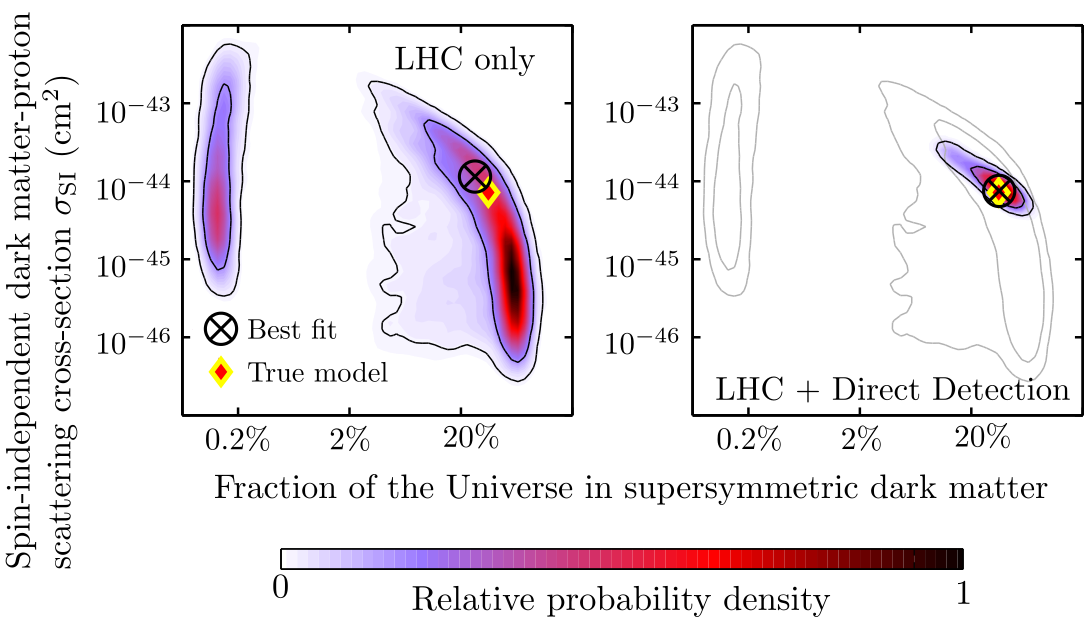
\includegraphics[width=1.35\linewidth]{Fig}
  \caption{An example of how a global fit can exploit the synergy between different experiments in the search for BSM physics and DM.  In the left panel, mock LHC data is used to try to identify an example supersymmetric model, in terms of the cosmological abundance of the DM and its scattering cross-section with protons.  Two main parameter regions are compatible with the mock data.  Shading indicates the relative probability of the different parts of the parameter space, and contours give $1\sigma$ and $2\sigma$ regions.  In the right panel, mock data from a direct search for DM is added to the global fit, breaking the degeneracy and providing a highly accurate reconstruction.  Here grey contours give the LHC-only result, for easy comparison.  Based on results from \cite{BertoneLHCDD}.}
  \label{example}
\end{SCfigure*}

\subsubsection*{Research Framework/Methodology}

The core methodology is that of a composite likelihood-based global fit (see e.g.~\cite{Trotta08,Akrami09,Scott09c}).  One first chooses a BSM physics scenario with some model parameters, and then calculates predicted experimental signatures of the model for arbitrary parameter combinations (gamma-ray fluxes, event rates at the LHC, etc).  Predictions are compared to experimental measurements, and a series of likelihood functions produced.

The likelihood describes the probability of obtaining the observed data if the BSM physics scenario is correct, given some combination of the model parameters.  Each experimental dataset has an associated likelihood function.  The individual likelihoods are multiplied to obtain a single combined likelihood.  By sampling the likelihood function at a number of different parameter combinations, one can map the overall likelihood surface.  This step is highly non-trivial and computationally intensive, even with sophisticated optimization algorithms \cite{Akrami09,SBspike}; traditional grid and random scans are woefully inadequate even for simple versions of the MSSM.  The samples are analysed with established statistical methods to produce likelihood maps and probability distributions for the different parameters and observables.  

An example of the utility of the global fit approach is shown in Fig.~\ref{example}.  Here probability distributions for the amount of supersymmetric DM, and its scattering cross-section with protons, are shown for two parameter scans.  In one scan (left), mock LHC data is used to try to `find' a particular example point in the parameter space of the MSSM.  Two broad regions of high probability exist, illustrating the model degeneracy with respect to LHC data alone.  When data from a future direct search for DM are added (right), the degeneracy is lifted, and the correct result is reconstructed with high accuracy.  Such analyses have the added advantage of being able to fully deal with uncertainties in modelling assumptions or standard input data, by including them as additional parameters in the fit.  The entire exercise can be repeated for different BSM scenarios with different parameterizations, and the results compared to determine if the data strongly favour one scenario over another.

In my analyses, likelihood functions will come from far and wide: Higgs and supersymmetry searches at the LHC and its predecessors \cite{ATLASHgammagamma11,ATLASSUSYljET11,CMSSUSYjET11a,CMSSUSYjET11b,ATLASmonojetET11}, low-energy accelerators \cite{HFAG07, CDFBmixinga, CDFBmixingb, CDFBmumu11}, the magnetic moment of the muon \cite{g-2}, beam dump/fixed target searches for light bosons \cite{Batell09,Bjorken09}, electroweak precision tests \cite{PDG}, DM direct detection experiments \cite{Bernabei08,CDMS2event,CDMSIILowE,XENON100,CoGeNTAnnMod11,CRESST11,SIMPLE11}, searches for antimatter in cosmic rays \cite{Pamelaantiproton10,Choutko02,Pamelaelectron11,Pamelapositron,AMSelectronpredict,Hailey09,Choutko08}, nuclear cosmic ray ratios \cite{CREAM1pHe}, radio data \cite{Regis08, Bergstrom09_MW}, effects of DM on reionisation \cite{Natarajan10,Cirelli09b}, recombination \cite{Slatyer09, Galli09} and helioseismology \cite{Taoso10}, the observed DM cosmological abundance \cite{WMAP7}, neutrino masses and mixings \cite{Schwetz11,Akhmedov10,Hamann10}, and other indirect DM searches \cite{IceCube09,Scott09c,LATcosmowimp,LATDwarfComposite,HESSdwarfs, MAGICSegue, VERITAS10}.  The latter part of my analysis will benefit greatly from directly collaborating with experiments: the IceCube neutrino telescope (via M.~Danninger, K.~Hultqvist and J.~Adams), the \emph{Fermi} gamma-ray space telescope (via J.~Conrad, T.~Jeltema, et al), and the VERITAS (\textit{via the McGill group of D.~Hanna and K.~Ragan}) and HESS/CTA (via J.~Conrad, J.~Ripken, et al) ground-based gamma-ray telescopes.

Not every dataset is relevant for all BSM scenarios.  I will confront a number of phenomenological incarnations of the MSSM with the data mentioned above, as well as some based on specific supersymmetry-breaking schemes.  DM-specific models will include simple effective DM, inert Higgs doublet models, asymmetric DM, inelastic/exciting models, isospin-violating DM and Sommerfeld enhanced models.  Many of the latter will be best implemented \textit{at McGill in close collaboration with Jim Cline}, as well as a global analysis of electroweak baryogenesis models and their implications for DM observables.  \textit{With a student at McGill (A.~Vincent)}, I have also begun investigating combined impacts of solar physics and laboratory experiments on axion-like and magnetic DM models.  Later (beyond the timeframe of this proposal), I intend to use global fit tools to investigate extensions to the MSSM, extra dimensional models, sterile neutrino DM, and left-right symmetric models.

This global fitting exercise will be done within the framework of three very large computer codes, designed to connect search algorithms, observable calculators and likelihood functions.  For DM-specific models, I will use \textsf{DMBayes}, a dedicated DM global-fitting package presently being developed by myself, R.~Trotta, R.~Ruiz de Austri and others.  Models with broader phenomenology will be analysed using \textsf{SuperBayeS} \cite{Ruiz06,Trotta08,SBweb}, a project on which I have also recently joined as an author, and later \textsf{SUFit}, a next-generation BSM global fit package I am developing in collaboration with others from the Oskar Klein Centre in Stockholm.  A key feature of \textsf{SUFit} is that it will allow extreme flexibility in switching between different BSM scenarios, likelihoods and observable calculators; this will be a key component in facilitating the very ambitious program I have laid out in this proposal.

\subsubsection*{Dissemination, Impact Enhancement and Spin-off Science}

I will disseminate the research by publishing it in top-tier journals like JCAP and JHEP, and presenting it at international conferences.

We intend to make the \textsf{DMBayes}, improved \textsf{SuperBayeS} and \textsf{SUFit} packages freely available to the community as open-source software.  This will hugely enhance the value and impact of the research of this proposal.  This includes the many instances of new and updated observable calculation routines contributing to the larger packages, many of which will see extensive use in the DM/phenomenology community outside the global fit arena.  A prime example is the set of IceCube codes currently being developed for use with \textsf{SuperBayeS} and \textsf{SUFit}, but planned for inclusion in the public version of \textsf{DarkSUSY} \cite{darksusy}.  Another example is the differential evolution algorithm discussed above, which will be released as a standalone public package.

Even after we fully characterize physics at the TeV scale, there will always be another energy frontier poorly constrained by data, as the TeV scale currently is.  It is in this environment that the technical details of the statistical treatment of global fits are most crucial.  The tools my collaborators and I develop for TeV-scale physics in the next few years, and the lessons we learn, will therefore also be directly applicable over the coming decades to the next era of particle physics.  \emph{Investment in this research program will therefore pay off not only in the cutting-edge research that it will produce in the two years of the fellowship, but for years to come.}

The research facilitated by the Banting Fellowship will also lead to substantial spin-off science.  The differential evolution package will be equally useful for cosmological parameter estimation (linked to e.g.~\textsf{CosmoMC} \cite{CosmoMC}), Galactic cosmic ray propagation (linked to e.g.~\textsf{USINE} \cite{Putze10}) and planet searches.  Our understanding of DM indirect detection places limits on the amplitude of cosmological perturbations via DM minihalos \cite{SS09,JG10,Bringmann11}, which in turn constrains models of inflation.  I intend to use the same techniques \textit{together with R.~Brandenberger at McGill} to place constraints on cosmic strings.  Eventually, where such early-Universe models have other observable consequences, the constraints may prove useful as additional likelihood components in global fits.  Similarly, one can use the global fit machinery to investigate inverse problems \cite{Roszkowski10,Akrami11DD}; one such problem is the ability of a SUSY detection at the LHC, coupled with the known cosmological abundance of DM, to constrain non-standard cosmologies and heavy moduli in the early Universe.  This is an avenue I will pursue \textit{with Wei Xue, a student at McGill}.

The IceCube and axion components of this proposal both depend upon the elemental composition of the Sun.  Having substantial experience in this field, together with M.~Asplund, N.~Grevesse and J.~Sauval \cite{ScottVII,Scott09Ni,AGSS}, I will continue to help refine our knowledge of this crucial input data.  I am also hopeful that the axion work might provide some clues as to why spectroscopy and helioseismology indicate different solar abundances.  Finally, DM can have a significant impact on stellar evolution, so investigating so-called `dark stars' \cite{Spolyar08,Iocco08a,Fairbairn08,Scott09,Zackrisson10a,Scott11} might also provide some complementary clues as to its identity.  This work will lead to yet further spin-offs, relating to the DM velocity distribution in the Galactic Centre (with R.~Church and M.~Davies) and core condensation in helium white dwarfs (with R.~Rosen \cite{Rosen08,Rosen10}).

\clearpage
\renewcommand\bibsection{}
\setcounter{page}{1}
\fancyhead[C]{Banting PDF -- Bibliography}
\bibliography{DMbiblio,SUSYbiblio,AbuGen,CosmoSF}

\end{document}
